% Generated 2021-02-25 22:49:50 +0530
\subsection{CuttingToolLifeCycle} \label{sec:CuttingToolLifeCycle}


This section provides the semantic information for the \block{CuttingToolLifeCycle} model.

\begin{figure}[ht]
  \centering
    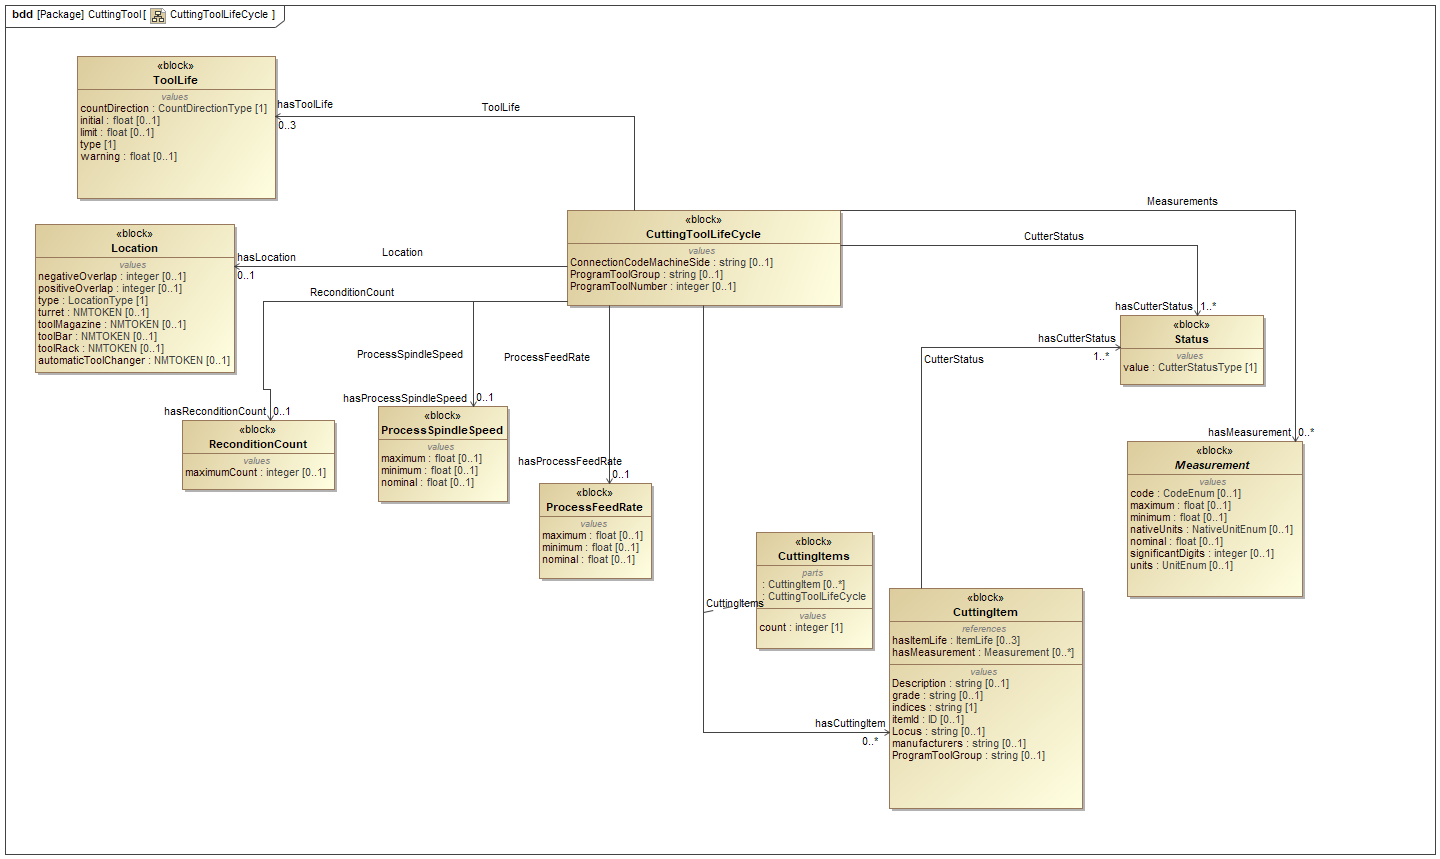
\includegraphics[width=1.0\textwidth]{figures/CuttingToolLifeCycle.png}
  \caption{CuttingToolLifeCycle Diagram}
  \label{fig:CuttingToolLifeCycle Diagram}
\end{figure}

\FloatBarrier


Note: See \sect{CuttingToolLifeCycle Schema Diagrams} for XML schema.



\subsubsection{CuttingToolLifeCycle}




Data regarding the application or use of the tool.

This data is provided by various pieces of equipment (i.e. machine tool, presetter) and statistical process control applications. Life cycle data will not remain static, but will change 395 periodically when a tool is used or measured.


\paragraph{Elements of CuttingToolLifeCycle}\mbox{}
\label{sec:Elements of CuttingToolLifeCycle}

\tbl{Elements of CuttingToolLifeCycle} lists the elements of \texttt{CuttingToolLifeCycle}.

\begin{table}[ht]
\centering 
  \caption{Elements of CuttingToolLifeCycle}
  \label{table:Elements of CuttingToolLifeCycle}
\tabulinesep=3pt
\begin{tabu} to 6in {|l|l|} \everyrow{\hline}
\hline
\rowfont\bfseries {Element} & {Multiplicity} \\
\tabucline[1.5pt]{}
\texttt{ConnectionCodeMachineSide} & 0..1 \\
\texttt{ProgramToolGroup} & 0..1 \\
\texttt{ProgramToolNumber} & 0..1 \\
\texttt{ProcessFeedRate} & 0..1 \\
\texttt{ToolLife} & 0..3 \\
\texttt{ProcessSpindleSpeed} & 0..1 \\
\texttt{Status} (organized by \block{CutterStatus}) & 1..* \\
\texttt{CuttingItem} (organized by \block{CuttingItems}) & 0..* \\
\texttt{Measurement} (organized by \block{Measurements}) & 0..* \\
\texttt{ReconditionCount} & 0..1 \\
\texttt{Location} & 0..1 \\
\end{tabu}
\end{table}
\FloatBarrier


Descriptions for elements of \block{CuttingToolLifeCycle}:

\begin{itemize}

\item \block{ConnectionCodeMachineSide} \newline Identifier for the capability to connect any Component of the cutting tool together, except Assembly Items, on the machine side. Code: CCMS

The value of \block{ConnectionCodeMachineSide} \MUST be \texttt{string}.

\item \block{ProgramToolGroup} \newline The tool group this tool is assigned in the part program.

The value of \block{ProgramToolGroup} \MUST be \texttt{string}.

\item \block{ProgramToolNumber} \newline The number of the tool as referenced in the part program.

The value of \block{ProgramToolNumber} \MUST be \texttt{integer}.

\item \block{ProcessFeedRate} \newline The constrained process feed rate for this tool in mm/s.

\item \block{ToolLife} \newline The cutting tool life as related to the assembly.

\item \block{ProcessSpindleSpeed} \newline The constrained process spindle speed for this tool.


\item \block{CutterStatus} \newline 

\item \block{CuttingItems} \newline \block{CuttingItems} \glspl{organize} \block{CuttingItem} elements.

\item \block{Measurements} \newline \block{Measurements} \glspl{organize} \block{Measurement} types.

\item \block{ReconditionCount} \newline The number of times this cutter has been reconditioned.


\item \block{Location} \newline The Pot or Spindle the cutting tool currently resides in.
\end{itemize}



\subsubsection{ToolLife}
\label{sec:ToolLife}



The cutting tool life as related to the assembly.


\paragraph{Attributes of ToolLife}\mbox{}
\label{sec:Attributes of ToolLife}

\tbl{Attributes of ToolLife} lists the attributes of \texttt{ToolLife}.

\begin{table}[ht]
\centering 
  \caption{Attributes of ToolLife}
  \label{table:Attributes of ToolLife}
\tabulinesep=3pt
\begin{tabu} to 6in {|l|l|l|} \everyrow{\hline}
\hline
\rowfont\bfseries {Attribute} & {Type} & {Multiplicity} \\
\tabucline[1.5pt]{}

\property{countDirection}[ToolLife] & \texttt{CountDirectionType} & 1 \\
\property{initial}[ToolLife] & \texttt{float} & 0..1 \\
\property{limit}[ToolLife] & \texttt{float} & 0..1 \\
\property{warning}[ToolLife] & \texttt{float} & 0..1 \\
\end{tabu}
\end{table}
\FloatBarrier

Descriptions for attributes of \block{ToolLife}:

\begin{itemize}

\item \property{countDirection}[ToolLife] \newline Indicates if the tool life counts from zero to maximum or maximum to zero.

\texttt{CountDirectionType} Enumeration:

\begin{itemize}
\item \texttt{UP} \newline The tool life counts up from zero to the maximum.
 
\item \texttt{DOWN} \newline The tool life counts down from the maximum to zero. 
\end{itemize}


\item \property{initial}[ToolLife] \newline The initial life of the tool when it is new.

\item \property{limit}[ToolLife] \newline The end of life limit for this tool.

\item \property{warning}[ToolLife] \newline The point at which a tool life warning will be raised.
\end{itemize}



\subsubsection{Location}
\label{sec:Location}



The Pot or Spindle the cutting tool currently resides in.


\paragraph{Attributes of Location}\mbox{}
\label{sec:Attributes of Location}

\tbl{Attributes of Location} lists the attributes of \texttt{Location}.

\begin{table}[ht]
\centering 
  \caption{Attributes of Location}
  \label{table:Attributes of Location}
\tabulinesep=3pt
\begin{tabu} to 6in {|l|l|l|} \everyrow{\hline}
\hline
\rowfont\bfseries {Attribute} & {Type} & {Multiplicity} \\
\tabucline[1.5pt]{}

\property{negativeOverlap}[Location] & \texttt{integer} & 0..1 \\
\property{positiveOverlap}[Location] & \texttt{integer} & 0..1 \\
\property{type}[Location] & \texttt{LocationType} & 1 \\
\property{turret}[Location] & \texttt{NMTOKEN} & 0..1 \\
\property{toolMagazine}[Location] & \texttt{NMTOKEN} & 0..1 \\
\property{toolBar}[Location] & \texttt{NMTOKEN} & 0..1 \\
\property{toolRack}[Location] & \texttt{NMTOKEN} & 0..1 \\
\property{automaticToolChanger}[Location] & \texttt{NMTOKEN} & 0..1 \\
\end{tabu}
\end{table}
\FloatBarrier

Descriptions for attributes of \block{Location}:

\begin{itemize}

\item \property{negativeOverlap}[Location] \newline The number of location at lower index values from this location.

\item \property{positiveOverlap}[Location] \newline The number of locations at higher index value from this location.


\item \property{type}[Location] \newline The type of location being identified. 

\texttt{LocationType} Enumeration:

\begin{itemize}
\item \texttt{POT} \newline The number of the pot in the tool handling system. 
\item \texttt{STATION} \newline The tool location in a horizontal turning machine. 
\item \texttt{CRIB} \newline The location with regard to a tool crib. 
\item \texttt{SPINDLE} \newline A location associated with a \gls{Spindle}. 
\item \texttt{TRANSFER\textunderscore POT} \newline A location for a tool awaiting transfer from a tool magazine to spindle or a turret. 
\item \texttt{RETURN\textunderscore POT} \newline A location for a tool removed from a \gls{Spindle} or turret and awaiting return to a tool magazine.
 
\item \texttt{STAGING\textunderscore POT} \newline A location for a tool awaiting transfer to a tool magazine or turret from outside of the piece of equipment. 
\item \texttt{REMOVAL\textunderscore POT} \newline A location for a tool removed from a tool magazine or turret awaiting transfer to a location outside of the piece of equipment.
 
\item \texttt{EXPIRED\textunderscore POT} \newline A location for a tool that is no longer usable and is awaiting removal from a tool magazine or turret. 
\item \texttt{END\textunderscore EFFECTOR} \newline A location associated with an end effector. 
\end{itemize}


\item \property{turret}[Location] \newline The turret associated with a tool.

\item \property{toolMagazine}[Location] \newline The tool magazine associated with a tool.


\item \property{toolBar}[Location] \newline The tool bar associated with a tool.

\item \property{toolRack}[Location] \newline The tool rack associated with a tool.

\item \property{automaticToolChanger}[Location] \newline The automatic tool changer associated with a tool.
\end{itemize}



\subsubsection{ReconditionCount}
\label{sec:ReconditionCount}



The number of times this cutter has been reconditioned.



\paragraph{Attributes of ReconditionCount}\mbox{}
\label{sec:Attributes of ReconditionCount}

\tbl{Attributes of ReconditionCount} lists the attributes of \texttt{ReconditionCount}.

\begin{table}[ht]
\centering 
  \caption{Attributes of ReconditionCount}
  \label{table:Attributes of ReconditionCount}
\tabulinesep=3pt
\begin{tabu} to 6in {|l|l|l|} \everyrow{\hline}
\hline
\rowfont\bfseries {Attribute} & {Type} & {Multiplicity} \\
\tabucline[1.5pt]{}

\property{maximumCount}[ReconditionCount] & \texttt{integer} & 0..1 \\
\end{tabu}
\end{table}
\FloatBarrier

Descriptions for attributes of \block{ReconditionCount}:

\begin{itemize}

\item \property{maximumCount}[ReconditionCount] \newline The maximum number of times this tool may be reconditioned.

\end{itemize}



\subsubsection{ProcessSpindleSpeed}
\label{sec:ProcessSpindleSpeed}



The constrained process spindle speed for this tool.



\paragraph{Attributes of ProcessSpindleSpeed}\mbox{}
\label{sec:Attributes of ProcessSpindleSpeed}

\tbl{Attributes of ProcessSpindleSpeed} lists the attributes of \texttt{ProcessSpindleSpeed}.

\begin{table}[ht]
\centering 
  \caption{Attributes of ProcessSpindleSpeed}
  \label{table:Attributes of ProcessSpindleSpeed}
\tabulinesep=3pt
\begin{tabu} to 6in {|l|l|l|} \everyrow{\hline}
\hline
\rowfont\bfseries {Attribute} & {Type} & {Multiplicity} \\
\tabucline[1.5pt]{}

\property{maximum}[ProcessSpindleSpeed] & \texttt{float} & 0..1 \\
\property{minimum}[ProcessSpindleSpeed] & \texttt{float} & 0..1 \\
\property{nominal}[ProcessSpindleSpeed] & \texttt{float} & 0..1 \\
\end{tabu}
\end{table}
\FloatBarrier

Descriptions for attributes of \block{ProcessSpindleSpeed}:

\begin{itemize}

\item \property{maximum}[ProcessSpindleSpeed] \newline The upper bound for the tool’s target spindle speed.

\item \property{minimum}[ProcessSpindleSpeed] \newline The lower bound for the tools spindle speed.


\item \property{nominal}[ProcessSpindleSpeed] \newline The nominal speed the tool is designed to operate at.
\end{itemize}



\subsubsection{ProcessFeedRate}
\label{sec:ProcessFeedRate}



The constrained process feed rate for this tool in mm/s.


\paragraph{Attributes of ProcessFeedRate}\mbox{}
\label{sec:Attributes of ProcessFeedRate}

\tbl{Attributes of ProcessFeedRate} lists the attributes of \texttt{ProcessFeedRate}.

\begin{table}[ht]
\centering 
  \caption{Attributes of ProcessFeedRate}
  \label{table:Attributes of ProcessFeedRate}
\tabulinesep=3pt
\begin{tabu} to 6in {|l|l|l|} \everyrow{\hline}
\hline
\rowfont\bfseries {Attribute} & {Type} & {Multiplicity} \\
\tabucline[1.5pt]{}

\property{maximum}[ProcessFeedRate] & \texttt{float} & 0..1 \\
\property{minimum}[ProcessFeedRate] & \texttt{float} & 0..1 \\
\property{nominal}[ProcessFeedRate] & \texttt{float} & 0..1 \\
\end{tabu}
\end{table}
\FloatBarrier

Descriptions for attributes of \block{ProcessFeedRate}:

\begin{itemize}

\item \property{maximum}[ProcessFeedRate] \newline The upper bound for the tool’s process target feedrate.

\item \property{minimum}[ProcessFeedRate] \newline The lower bound for the tools feedrate.

\item \property{nominal}[ProcessFeedRate] \newline The nominal feedrate the tool is designed to operate at.

\end{itemize}



\subsubsection{Status}
\label{sec:Status}



The status of the cutting tool.


The value of \texttt{Status} \MUST be \texttt{CutterStatusType}.



\subsubsection{Measurement}
\label{sec:Measurement}



A constrained scalar value associated with a cutting tool.


\texttt{code}: \texttt{}.


\paragraph{Attributes of Measurement}\mbox{}
\label{sec:Attributes of Measurement}

\tbl{Attributes of Measurement} lists the attributes of \texttt{Measurement}.

\begin{table}[ht]
\centering 
  \caption{Attributes of Measurement}
  \label{table:Attributes of Measurement}
\tabulinesep=3pt
\begin{tabu} to 6in {|l|l|l|} \everyrow{\hline}
\hline
\rowfont\bfseries {Attribute} & {Type} & {Multiplicity} \\
\tabucline[1.5pt]{}

\property{maximum}[Measurement] & \texttt{float} & 0..1 \\
\property{minimum}[Measurement] & \texttt{float} & 0..1 \\
\property{nativeUnits}[Measurement] & \texttt{NativeUnitEnum} & 0..1 \\
\property{nominal}[Measurement] & \texttt{float} & 0..1 \\
\property{significantDigits}[Measurement] & \texttt{integer} & 0..1 \\
\property{units}[Measurement] & \texttt{UnitEnum} & 0..1 \\
\end{tabu}
\end{table}
\FloatBarrier

Descriptions for attributes of \block{Measurement}:

\begin{itemize}

\item \property{code}[Measurement] \newline A shop specific code for this measurement. ISO 13399 codes \textbf{MAY} be used for these codes as well. 

See \sect{CuttingTool Measurement Types} and \sect{CuttingItem Measurement Types} for details on \block{Measurement} types and their respective \property{code} values.

\item \property{maximum}[Measurement] \newline The maximum value for this measurement. 

\item \property{minimum}[Measurement] \newline The minimum value for this measurement. 

\item \property{nativeUnits}[Measurement] \newline The units the measurement was originally recorded in.

\item \property{nominal}[Measurement] \newline The as advertised value for this measurement.


\item \property{significantDigits}[Measurement] \newline The number of significant digits in the reported value. 

\item \property{units}[Measurement] \newline The units for the measurements. 
\end{itemize}


